% !TeX root = Report.tex

\documentclass[12pt]{article}
% include enumitem
\usepackage{enumitem}
\usepackage{listings}
\usepackage{sectsty}
\usepackage{color}
\usepackage{float}
\restylefloat{table}
\usepackage{graphicx}
\usepackage{biblatex}

\usepackage{changepage}

\usepackage{xcolor}
\usepackage{listings}

\addbibresource{Library2.bib}

\title{GoodDNS: A Good DNS Server}
\date{\today}

\graphicspath{ {./images/} }

\begin{document}

\subsectionfont{\fontsize{12}{14}\selectfont}

\maketitle

\tableofcontents

\section{Introduction}

\subsection{Overview}
GoodDNS is a simple yet efficient DNS\cite{DomainNamesImplementation1987} (Domain Name System) server that can be used to resolve domain names to IP\cite{InternetProtocol1981} (Internet Protocol) addresses. It is written in C\# and utilizes only stock libraries.
The server adheres strictly to the protocol as defined in RFC 1035\cite{DomainNamesImplementation1987}. This report will describe the implementation and
development of GoodDNS, as well as the challenges faced during development.

\subsection{Domain Name System}
The Domain Name System\cite{DomainNamesImplementation1987} is a system described in RFC 1035\cite{DomainNamesImplementation1987} 
that is used to resolve domain names to IP addresses. The domain name system is hierarchical, each domain name server relies on higher level domain name servers to resolve domain names.
GoodDNS is a recursive DNS server, meaning that it will resolve domain names by querying other DNS servers. But it also supports defining authorative DNS records for lower level subdomains.
This is a neat feature that allows the user to define custom DNS records for their own domain names.

\subsection{DNS Records}
The DNS\cite{DomainNamesImplementation1987} system uses DNS\cite{DomainNamesImplementation1987} records to store information about domain names. 
Here is a list of the most commonly used DNS records:
\begin{itemize}
    \item \textbf{A}: Stores an IPv4 address
    \item \textbf{AAAA}: Stores an IPv6 address
    \item \textbf{CNAME}: Stores a canonical name for an alias
    \item \textbf{MX}: Stores a mail exchange record
    \item \textbf{NS}: Stores an authoritative name server
    \item \textbf{PTR}: Stores a pointer to a canonical name
    \item \textbf{SOA}: Stores the start of a zone of authority
    \item \textbf{SRV}: Stores service location
    \item \textbf{TXT}: Stores text information
\end{itemize}
Some noteworthy DNS records are the \textbf{A} record, which stores an IPv4 address, and the \textbf{AAAA} record, which stores an IPv6 address. 
These records are used to resolve domain names to IP addresses. The \textbf{NS} record is also noteworthy, as this is the record that is used
to define authorative DNS servers on another domain name server. This is how the DNS system is hierarchical, each domain name server
relies on higher level domain name servers to resolve domain names.

\subsection{RFC 1035}
RFC 1035\cite{DomainNamesImplementation1987} are the specifications that define how the Domain Name System operates. 
RFC stands for Request For Comments, and is a document that describes a standard or protocol.
All commonly used protocols have an RFC document that describes how they operate.

\subsection{UML}
An UML\cite{UnifiedModelingLanguage} diagram is a diagram that describes the structure of a system. UML stands for Unified Modeling Language, 
and is a set of strict specifications that describe how UML diagrams should be structured. The specifications are designed by the 
Object Management Group\cite{https://themeforest.net/user/dan_fisherOMGObjectManagement} (OMG). UML diagrams are designed to be language agnostic, and
can be used to describe the structure of any system. The UML diagram for GoodDNS can be found in \textit{Figure \ref{fig:uml}}, this diagram describes the 
class relationships in GoodDNS. There are also many other types of UML diagrams, such as sequence diagrams, which describe the flow of a system.

\subsection{SOLID Principles}
The SOLID\cite{SOLID2023} priniciples is an acronym for five commonly adopted design principles in the design of object oriented software.
The SOLID principles are:
\begin{itemize}
    \item \textbf{S}ingle Responsibility Principle
    \item \textbf{O}pen/Closed Principle
    \item \textbf{L}iskov Substitution Principle
    \item \textbf{I}nterface Segregation Principle
    \item \textbf{D}ependency Inversion Principle
\end{itemize}
The SOLID principles were first introduced by Robert C. Martin in his 2000 paper 
\textit{Design Principles and Design Patterns}\cite{martinDesignPrinciplesDesign2000}.
It is worth mentioning that the SOLID principles are not the only design principles that exist, but they were some 
of the first design principles to be introduced, and are still widely used today. Some competing design principles includes
the CUPID\cite{CUPIDJoyfulCoding2022}, and GRASP\cite{GRASPObjectorientedDesign2023} principles. This project loosely 
follows the SOLID principles as well as the CUPID\cite{CUPIDJoyfulCoding2022} principles.

\section{Domain Name System}
This section will describe the Domain Name System and how it operates.
We will also cover how parts of the Domain Name System are implemented in GoodDNS.

\subsection{DNS Architecture}
In RFC 1035\cite{DomainNamesImplementation1987} the Domain Name System is described as a hierarchical system of domain name servers.
RFC 1035\cite{DomainNamesImplementation1987} provides us with a very detailed description of how the Domain Name System operates.
The following are some illustrations of the Domain Name System architecture, as described in RFC 1035\cite{DomainNamesImplementation1987}.

The domain name system consists of many domain name servers, each domain name server is responsible for a zone of authority.
A zone of authority is a domain name, and all subdomains of that domain name. For example .com is a zone of authority, and example.com is a subdomain of .com.
GoodDNS is designed to be the zone of authority for third level subdomains, such as example.com. This means that GoodDNS is responsible for resolving
domain names such as www.example.com, but not example.com. This is because example.com is a second level subdomain, and GoodDNS is only responsible for 
third level subdomains see \textit{Figure \ref{fig:NS}}.

\begin{figure}[h]
    \begin{lstlisting}
        QUERY 1                         QUERY 2
                        +--------+
         example.com    | Client |       www
                        +--------+       
            |   A                       |   A   
            |   |                       |   |
            |   |                       |   |
            V   |                       V   |
    +--------------------+       +--------------------+
    | Foreign DNS Server |       | GoodDNS Server     |
    +--------------------+       +--------------------+
    
    \end{lstlisting}
    \caption{A foreign DNS server refering a client to GoodDNS}
    \label{fig:NS}
\end{figure}

\subsection{Recursive DNS}
GoodDNS is a recursive DNS server, this means that if it is not the zone of authority for a domain name, 
it will query other DNS servers to resolve the domain name. This is what allows the DNS system to be hierarchical.
This is also what allows GoodDNS to resolve domain names that it is not the zone of authority for, by relaying the query to other DNS servers and 
caching the result. See \textit{Figure \ref{fig:recursive}}.

\begin{figure}[h!]
\begin{lstlisting}
+--------------------+
| Foreign DNS Server |
+--------------------+       query
          |               <-----------------+
          |                
+--------------------+       +--------------------+
| Foreign DNS Server |       | GoodDNS Server     |
+--------------------+       +--------------------+
          |                  response
          |              +----------------->
+--------------------+    
| Foreign DNS Server |
+--------------------+
\end{lstlisting}
\caption{recursive DNS query from GoodDNS to foreign DNS servers}
\label{fig:recursive}
\end{figure}

\subsection{DNS packets}
A DNS packet consists of a header, a question, an answer, an authority and an additional section.
In this section we will describe the structure of the header, question and answer sections of a DNS packet.
We are not going to cover the authority and additional sections, as these are not used by GoodDNS.
see \textit{Figure \ref{fig:packet}} for a quick overview of the DNS packet structure.
\\
\\
\\
\\
\\
\\
\\
\\

\begin{figure}[h]
    \begin{lstlisting}
+---------------------+
|        Header       |
+---------------------+
|       Question      | The question for the name server
+---------------------+
|        Answer       | RRs answering the question
+---------------------+
|      Authority      | RRs pointing toward an authority
+---------------------+
|      Additional     | RRs holding additional information
+---------------------+
    \end{lstlisting}
    \caption{a quick overview of the DNS packet structure}
    \label{fig:packet}
\end{figure}


\subsection{DNS Header}
The DNS header is the first section of a DNS packet. It contains the following fields as shown in \textit{Figure \ref{fig:header}}:
\textbf{ID}: A 16 bit identifier assigned by the program that generates any kind of query. This identifier is copied
the corresponding reply and can be used by the requester to match up replies to outstanding queries.
\textbf{QR}: A one bit field that specifies whether this message is a query (0), or a response (1).
\textbf{Opcode}: A four bit field that specifies kind of query in this message.
\textbf{AA}: Authoritative Answer - this bit is valid in responses, and specifies that the responding name server is an authority 
for the domain name in question section.
\textbf{TC}: TrunCation - specifies that this message was truncated due to length greater than that permitted on the transmission channel.
\textbf{RD}: Recursion Desired - this bit may be set in a query and is copied into the response. If RD is set, it directs the name server
to pursue the query recursively.
\textbf{RA}: Recursion Available - this be is set or cleared in a response, and denotes whether recursive query support is available in the name server.
\textbf{Z}: Reserved for future use. Must be zero in all queries and responses.
\\
The rest of the fields represent the number of entries in the question, answer, authority and additional sections of the DNS packet.
\begin{figure}
\begin{lstlisting}
+--+
|ID|
+--+------+--+--+--+--+--+--+--+
|QR|Opcode|AA|TC|RD|RA| Z|AD|CD|
+--+------+--+--+--+--+--+--+--+
|           QDCOUNT            |
+--+--+--+--+--+--+--+--+--+--+
|           ANCOUNT            |
+--+--+--+--+--+--+--+--+--+--+
|           NSCOUNT            |
+--+--+--+--+--+--+--+--+--+--+
|           ARCOUNT            |
+--+--+--+--+--+--+--+--+--+--+
\end{lstlisting}
\caption{a quick overview of the DNS header structure}
\label{fig:header}
\end{figure}

\subsection{DNS Question}
The DNS question is the second section of a DNS packet. It contains the following fields as shown in \textit{Figure \ref{fig:header}}:
\textbf{QNAME}: a domain name represented as a sequence of labels, where each label consists of a length octet (4 bit) followed by that number of octets.
\textbf{QTYPE}: a two octet code which specifies the type of the query.
\textbf{QCLASS}: a two octet code that specifies the class of the query.
see \textit{Figure \ref{fig:question}} for a quick overview of the DNS question structure.
\\
\\
\\
\\
\\
\\
\\
\\
\\
\\
\\
\\

\begin{figure}
\begin{lstlisting}
+--+--+
|QNAME| a domain name represented as a sequence of labels,
+--+--+ where each label consists of a length octet followed
|QTYPE| by that number of octets.
+--+--+-+
|QCLASS | a two octet code that specifies the class of the query.
+--+--+-+
\end{lstlisting}
\caption{a quick overview of the DNS question structure}
\label{fig:question}
\end{figure}

\subsection{DNS Answer}
The DNS answer is the third section of a DNS packet. It contains the following fields as shown in \textit{Figure \ref{fig:answer}}:
\textbf{NAME}: a domain name to which this resource record pertains.
\textbf{TYPE}: two octets containing one of the RR (Resource Record) TYPE codes.
\textbf{CLASS}: two octets which specify the class of the data in the RDATA field.
\textbf{TTL}: a 32 bit unsigned integer that specifies the time interval that the resource record may be cached before the source of the information should again be consulted.
\textbf{RDLENGTH}: an unsigned 16 bit integer that specifies the length in octets of the RDATA field.
\textbf{RDATA}: a variable length string of octets that describes the resource.
see \textit{Figure \ref{fig:answer}} for a quick overview of the DNS answer structure.
\\
\\
\\
\\
\\
\\
\\
\\
\\
\\
\\
\\

\begin{figure}[h]
    %make font smaller for this figure
    \begin{lstlisting}[basicstyle=\tiny]
+--+-+
|NAME| a domain name to which this resource record pertains.
+--+-+
|TYPE| two octets containing one of the RR TYPE codes.
+--+-+
|CLASS| two octets which specify the class
+---+   of the data in the RDATA field.
|TTL| a 32 bit unsigned integer that specifies the time interval that the resource
+---+----+ record may be cached before the source of the information should again be consulted.
|RDLENGTH| an unsigned 16 bit integer that specifies the length in octets of the RDATA field.
+---+-+--+
|RDATA| a variable length string of octets that describes the resource.
+---+-+
    \end{lstlisting}
\caption{a quick overview of the DNS answer structure}
\label{fig:answer}
\end{figure}

\section{Architecture}
    The general architecture of GoodDNS can be divided into three main components:
    \begin{itemize}
        \item Presentation Layer
        \item Application Layer
        \item Data Layer
    \end{itemize}

    \subsection{Presentation Layer}
    The presentation layer is the layer that the user interacts with. In GoodDNS, the presentation layer consists of the settings class,
    and the logging class. The settings class is used to read settings specified by the user. Such as the port numbers for the TCP and UDP servers.
    The logging class is used to log information to the console and to the log file, such as when the server starts, or when a DNS query is received.

    \subsection{Application Layer}
    The application layer is the layer that contains the business logic of the application. In GoodDNS, 
    the application layer consists of the following classes:

    \subsubsection{Packet}
    This class is used to represent a DNS packet. It contains methods for parsing and serializing DNS packets.
    \subsubsection{Question}
    When the packet parser reaches the first question in the DNS class, controll of the data pointer is passed to the question class.
    \subsubsection{Answers}
    When the packet parser reaches the first answer in the DNS class, controll of the data pointer is passed to the answer class.
    \subsubsection{Flagpole}
    The packet creates an instance of the flagpole class, and passes it all relevant flags. 
    The flagpole class is used to store the flags of the DNS packet.
    \subsubsection{Server}
    This is an interface for the TCP and UDP servers. It contains methods for starting and stopping the server. 
    Thus making the server logic protocol agnostic.
    \subsubsection{UDP Server}
    This class instanciates lots of UDP listeners, and creates new working threads for each user session.
    \subsubsection{TCP Server}
    This class instanciates lots of TCP listeners, and creates new working threads for each user session.
    \subsubsection{Universal Client}
    This class is used as a protocol agnostic interface for the packet recieved callback. Thus making the server logic protocol agnostic.
    \\
    \\
    \subsection{Data Layer}
    The data layer is responsible for caching, reading and recieving DNS records. In GoodDNS, the data layer consists of the following classes:
    \subsubsection{BIND}
    This class is used to read Zone\cite{ZoneFile2023} files. It contains methods for reading and parsing Zone files.
    \subsubsection{Cache}
    This class is used to cache DNS records. It contains methods for adding, removing and retrieving DNS records.
    \subsubsection{Record Requester}
    This class is creates and manages different transactions to other DNS servers. It contains methods for creating and managing transactions.
    \subsubsection{Transaction}
    The transaction contains the logic for sending and recieving DNS questions and answers. It is what allows the DNS server to be recursive.
    \\
    \\
    The relationships between these classes can be seen in \textit{Figure \ref{fig:uml}}.
    \\
    \\

\begin{figure}[h!t]
    % Adjust margins for this figure
    \begin{adjustwidth}{-1in}{-1in}
      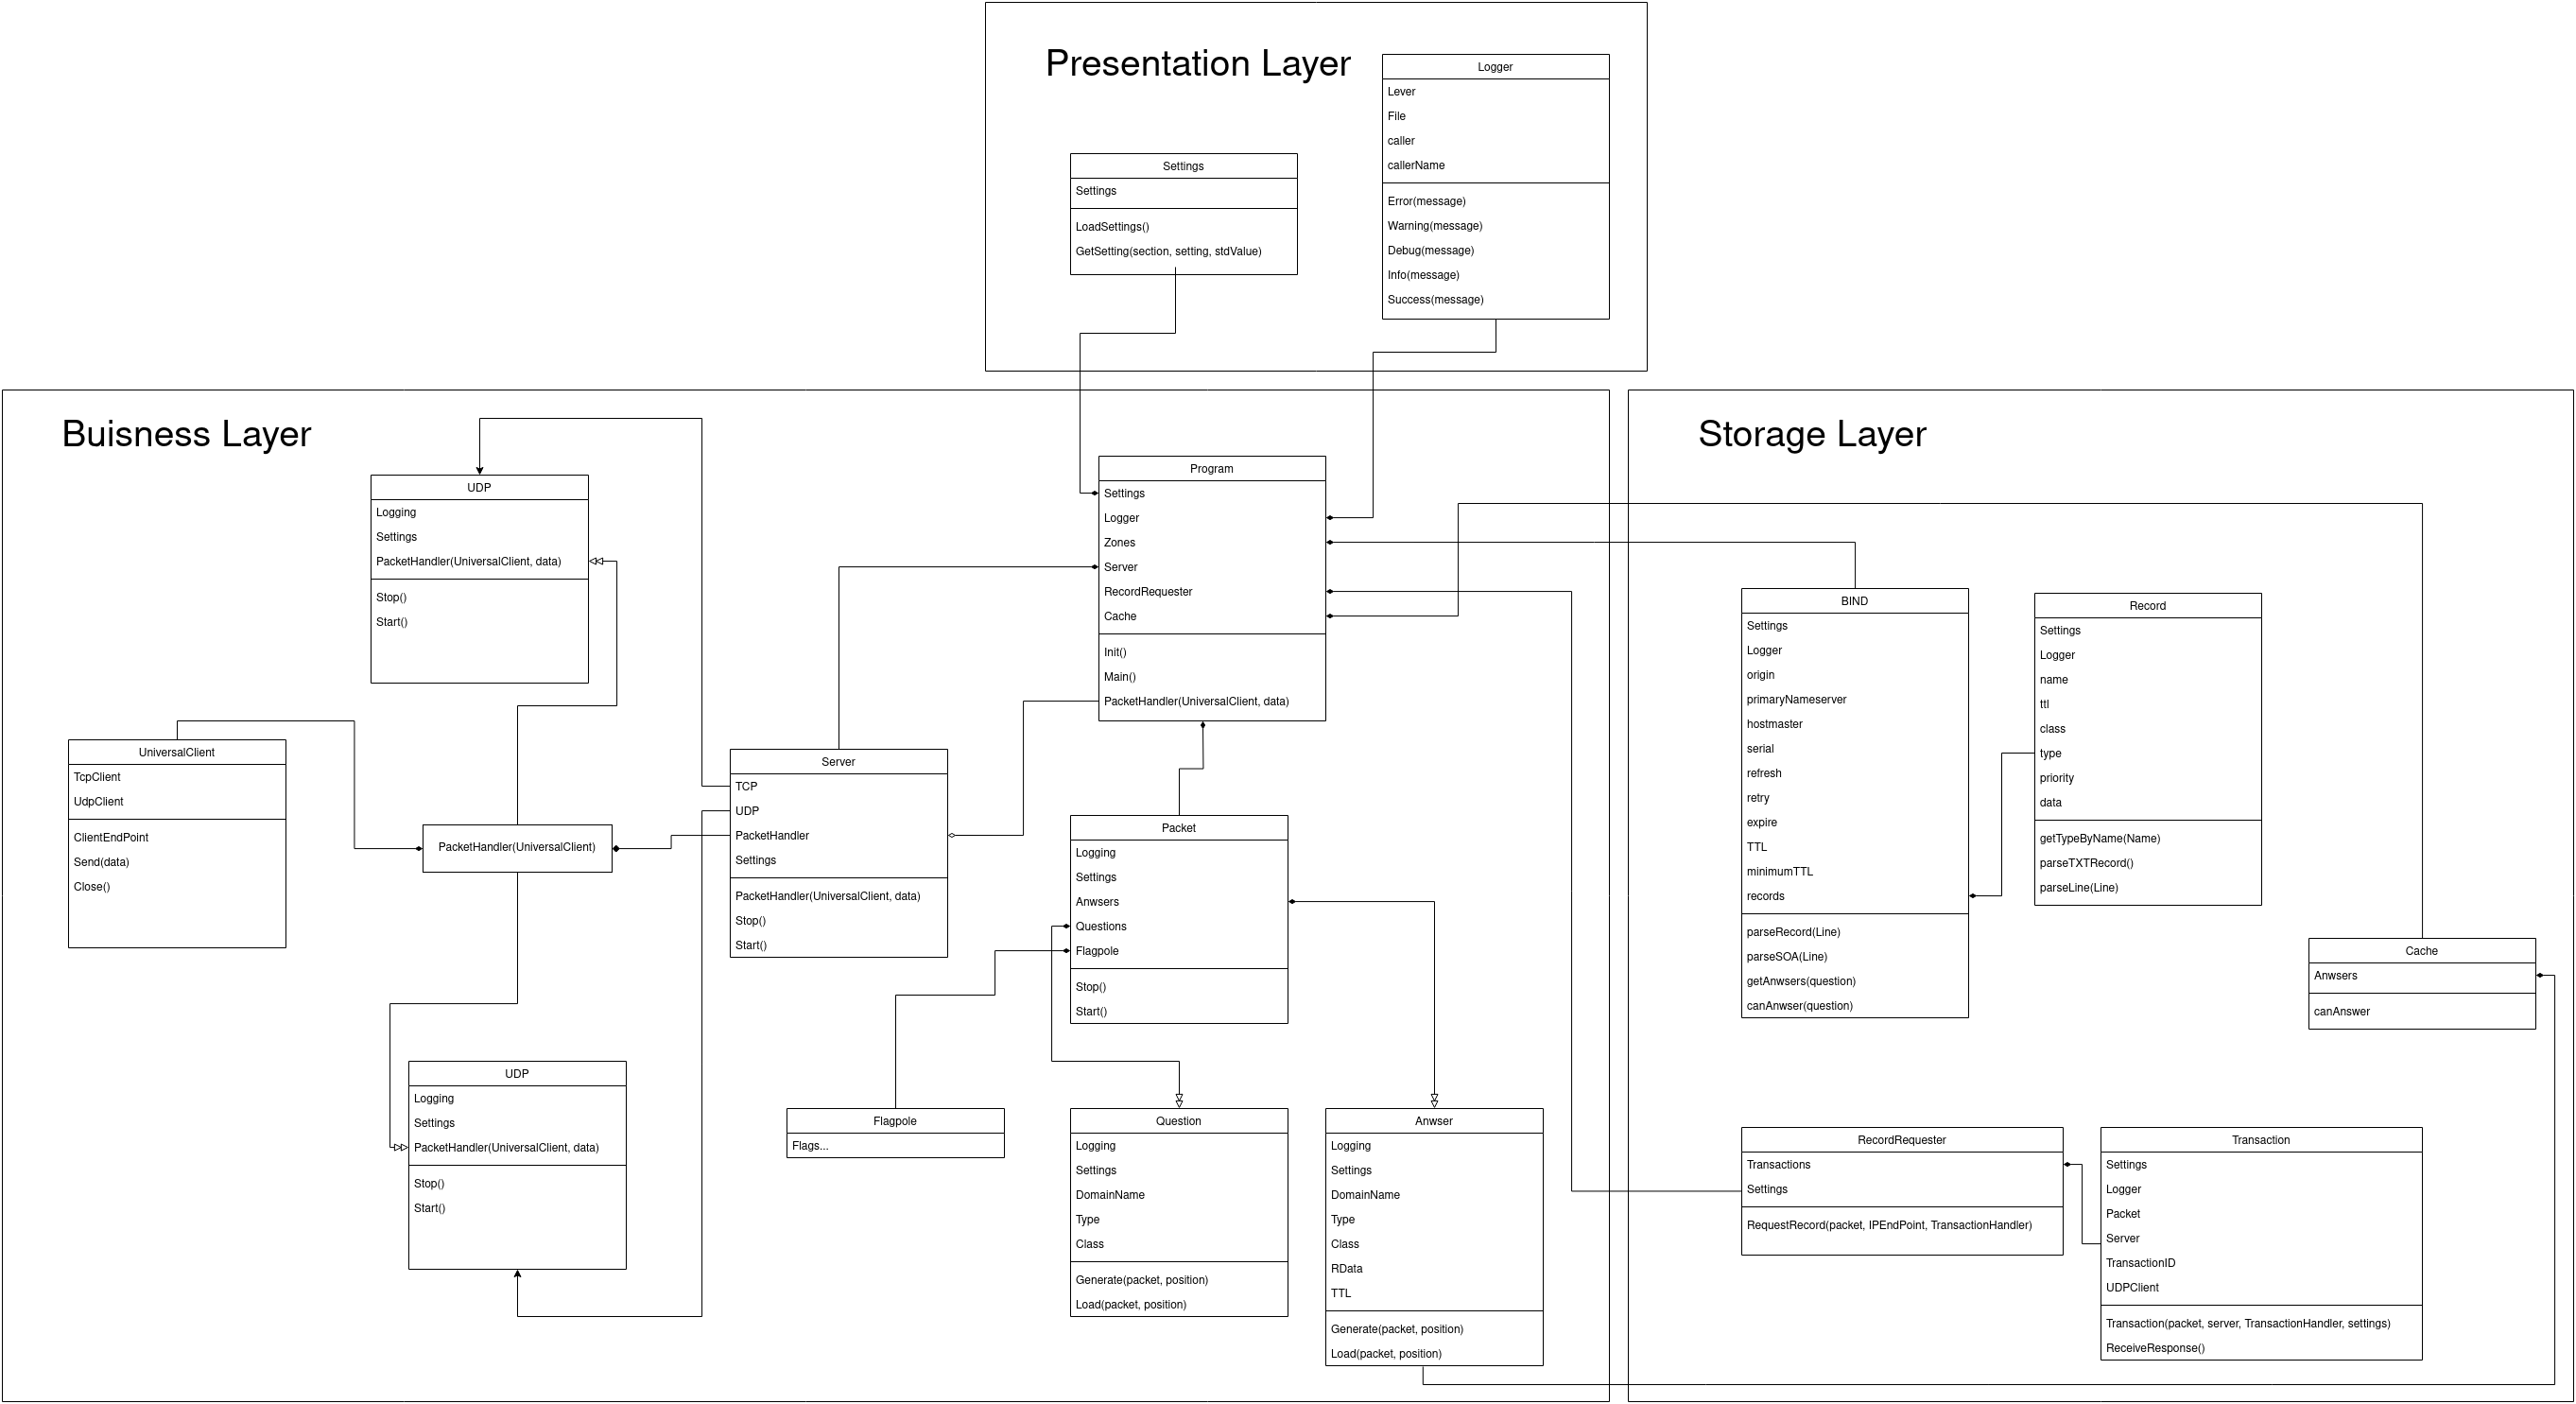
\includegraphics[width=\linewidth]{uml3.drawio.png}
      \caption{UML Diagram}
      \label{fig:uml}
    \end{adjustwidth}
\end{figure}
\clearpage

\subsection{The utilization of SOLID principles}
All classes follow the single responsibility principle, and the open/closed principle.
The adhereance to the single responsibility principle could be improved by abstracting the parsing and serializing of data into its own
protocol agnostic template class, this would allow to easily define packet structures using a set of arbitrary instructions.

The program adheres to the Open Closed principle, this is achieved trough the callback system used by the TCP, UDP Server and Resource Requester.
The program also theoretically adheres to the Liskov Substitution principle, but due to the program only implementing one byte protocol there is
no need to inherit from abstract or allready existing classes.

The adhereance to the interface segregation principle can be seen in the use of the server interface, which is used to abstract the TCP and UDP servers.
It can also be seen in the use of the Universal Client class, which is used to abstract the process of responding to a DNS query.

The dependency inversion principle is adhered to by the use of dependency injection. This allows for a loose coupling between the settings class
and the rest of the program. The callbacks are also a sort of dependency injection which removes the higher level packet processing logic from the 
lower lever server logic.

\subsection{Commonly used design patterns}

The settings class is implemented following the singleton design pattern, 
a quite logical choice since there is no need for multiple instances of the settings class. 
The logger class does not adhere to the singleton design pattern, 
allowing different parts of the program to execute distinct levels of logging to different log files.

Within the program, there are also instances of factories, 
such as the question parsing methods within the packet class and the BIND (Zone file) parser, utilized for generating DNS records.

The program heavily relies on callbacks, this adheres to the observer design pattern.
The combination of callbacks and lambda expressions enhances code readability and cleanliness.

Dependency injection is utilized to propagate the settings class throughout the program. 
Additionally, callbacks serve as a form of dependency injection, 
separating the higher-level packet processing logic from the lower-level server logic. 
This modular approach contributes to a more maintainable and flexible codebase.


\subsection{Event driven architecture}
The programs is built around a simple yet solid event driven architecture, this allows the program to handle multiple clients simultaneously.
The core mechanisme of this architecture is the creation of a working thread for each client. This contributes to the scalability of the program.

When a DNS query is received the program will dynamically initiate a new working thread, and pass the DNS query to this thread.
This enables the program to handle multiple clients simultaneously. The working thread will then instansiates a new Universal Client, this 
client encapsulates all data needed to respond to the query, this is also what allows the rest of the program to be protocol agnostic.

The Universal Client will then be passed to a callback method, this callback method is what disconnects the higher level packet processing logic
from the lower level server logic. The callback also provides the higher level processing its own working thread, this allows the program to handle
multiple clients simultaneously. This is the core mechanisme of the event driven architecture. And this is what allows the program to scale so efficiently.


\section{Development}
\subsection{Version Control}
Version control systems are used to track changes in a set of files. This project relies
on the version control system Git\cite{Git} to track changes in the source code. Git is a distributed version control system,
meaning that each user has a local copy of the repository (A collection of files tracked by Git), and can make changes to this local copy.
These changes can then be pushed to a Git server containing the main repository. This allows for multiple users to work on the same project

\subsubsection{Branches}
A branch is a copy of the repository. Branches allows us to simultaneously work on different features of the program without interfering with each other.
GoodDNS uses a system called feature branches, where each branch is named after the feature that is being implemented.
When a feature is completed, the branch is merged into the main branch.
Working versions of the main branch can be branched of to the release branch, which always contains a working version of the program.
This system creates some challenges during major refactoring, as this will break all other branches. 
This is why major refactoring should be done on the main branch.

\subsubsection{Testing}
Integration testing is a method of testing different components of a system together. GoodDNS uses integration testing to 
test the following components:
\begin{itemize}
    \item The UDP server
    \item The TCP server
    \item The BIND\cite{ZoneFile2023} class
\end{itemize}

The tests establish a DNS server, and then sends a DNS query to this server. The test then checks if the server responds with the correct DNS record.
This is a very simple yet effective way of testing the system. The tests are configured to run automatically each time a commit is pushed to the Git server.
More tests can easily be added due to the modular nature of the program.

\subsection{Refactoring}
The way the program handles the byte data found in the DNS queries were refactored multiple times during development.
This area could still be improved like mentioned in the SOLID principles section. There were also a lot of styling changes during development,
as the codebase was not very consistent in the beginning. The codebase is now much more consistent, and the adhereance to C\# coding conventions\cite{billwagnerNETDocumentationCoding2023} is
more strict.

\section{Usage}
\subsection{Settings}
The server expects a configuration file named \textit{settings.ini} to be present in the same directory as the executable.
the settings file should look like this:
\begin{lstlisting}
    [logging]
    path=./log.txt; the path to the log file.
    logLevel=1; the log level, 0 is no logging, 1 is info logging, 
    ;2 is debug logging... 5 is warning logging.
    [server]
    port=54321; this port is used for both TCP and UDP,
    ;note DNS usually uses port 53.
    tcpThreads=10; the amount of threads allowed to be 
    ;used by the TCP server.
    udpThreads=10; the amount of threads allowed to be 
    ;used by the UDP server.
    [requester]
    server=1.1.1.1; the DNS server to use for 
    ;recursive DNS queries.
    path=./zones; the path to the zone files.
\end{lstlisting}
All settings have a standard parameter and will run with the settings above if no settings file is found.

\subsection{Zone files}
The server expects zone files to be present in the directory specified by the \textit{path} parameter in the settings file.
A zone file should look like this:
\begin{lstlisting}
    $ORIGIN example.com.
    @ SOA ns1.example.com.  (
        hostmaster.example.com. ; hostmaster email address
        2018080801 ; serial
        28800      ; refresh
        7200       ; retry
        864000     ; expire
        86400      ; minimum
    )
    www 60 A xxx.xxx.xxx.xxx
\end{lstlisting}
The zone file above defines the domain name \textit{example.com} and the subdomain \textit{www.example.com}.

\printbibliography

\end{document}